
\chapter{Scope}
Die Moduldokumentation beschreibt die Architektur, die Schnittstellen 
und die Hauptmerkmale des Moduls. Außerdem werden die Modul bzw. Komponententests 
einschließlich der Ergebnisse beschrieben und dokumentiert. 
Die MOD dient bei Bedarf auch als Programmier- oder Integrationshandbuch für das 
Modul. Wenn bestimmte Risiken direkt mit der Verwendung des Moduls verknüpft sind,
so sind sie in diesem Dokument zu benennen und zu kommentieren.
\\
Dieses Modul hat die Aufgabe, Byte Buffer aus UDP Streams in Objekte zu transformieren und umgekehrt.
Es ist folglich nur für die Erstellung und das Parsen von Paketen zuständig.
Das Empfangen oder Versenden von Paketen ist nicht Teil der Funktionalität dieses Moduls.

\chapter{Definitionen}

\section{Abkürzungen}

GUI - Graphical user Interface  \\
UDP - User Datagram Protocol \\
IP - Internet Protocol \\
TCP - Transmission Control Protocol
\section{Definitionen}
%Wichtige Begriffe und Worte

\paragraph{Maven} Ein Build-Management-Tool der Apache Software Foundation und basiert auf
Java. Mit ihm kann man insbesondere Java-Programme standardisiert erstellen und
verwalten.
\paragraph{Sonar} Sonar vereint die Funktionen von diverser Tools zur statischen Code-Analyse
unter einem Dach und bietet eine komfortable Web-Oberfläche zur Auswertung der
gesammelten Statistiken an.

\chapter{Analyse}

\section{Voruntersuchungen}
%Müssen/mussten Prototypen gemacht werden?
%Versuche, Test und Abschätzungen 

Der endgültigen Paket Spezifikation und Implementierung gingen zahlreiche Voruntersuchungen, Abschätzungen und Evaluationen voraus.
Um ein Paketformat zu spezifizieren, ist es von größter Relevanz, genau zu wissen wie dieses transportiert wird und welche Annahmen über das System getroffen werden können. So stellen sich folgende Fragen

\begin{enumerate}
\item Können Pakete explizit verschickt werden oder stellt sich die Übertragung für den Benutzer als Stream dar?
\item Werden Pakete garantiert übermittelt?
\item Können übermittelte Pakete verfälscht werden?
\item Gibt es Größenbeschränkungen für Pakete?
\item Wie werden Pakete geroutet? Müssen hier Besonderheiten beachtet werden?
\item Wie viele Möglichkeiten bietet das Framework? Kann auch auf untere Schichten des Netzwerk Stacks zugegriffen werden?
\item Wie viele Pakete können pro Zeiteinheit Übertragen werden?
\item Ist es schneller wenige große oder viele kleine Pakete zu Übertragen?
\end{enumerate}

Um diese Fragen zu beantworten, wird der direkte technische Kontext in den folgenden Abschnitten erläutert.
Zu diesem Kontext gehören vor Allem die Java-Plattform
und die Multicasting-Fähigkeit des Internet Protocol (IP). Um den Kontext zu
strukturieren kommt hier das (eher theoretische) OSI-Schichtenmodell und dessen
in der Praxis angewandte Umsetzung, das TCP/IP-Modell, zum Einsatz.

\subsection{Logische Funktionsweise}

Die von der Software getestete Multicasting-Technologie ist optionaler
Bestandteil des Internet Protocol. In einer IP-Umgebung, die Multicasting
unterstützt, können damit Pakete an mehrere Empfänger gleichzeitig gesendet
werden, ohne dass vom Sender zu jedem einzelnen Empfänger eine eigene Verbindung
aufgebaut werden muss. Außerdem muss ein Paket, das mehrere Empfänger erreichen
soll, trotzdem nur ein einziges Mal vom Sender versendet werden.\\
\\
Der Netzerkverkehr wird beim Multicasting in \emph{Multicast-Gruppen}
organisiert. Alle Endgeräte, die die Multicasting-Pakete eines bestimmten
Senders empfangen möchten, treten einer bestimmten Multicast-Gruppe bei.
Andersherum sendet ein Host, der Multicast-Pakete verschickt, diese nicht an
eine "`gewöhnliche"' IP-Adresse, die einen bestimmten Host identifizieren würde,
sondern an eine \emph{Multicast-Adresse}. Für Multicast-Adressen wurden eigens
bestimmte IP-Adressblöcke reserviert. Jede Multicast-Adresse steht für eine
Multicast-Gruppe. In diesem Sinne wird eine Multicast-Gruppe "`eröffnet"', indem
mindestens ein Host mindestens ein Paket an ihre IP-Adresse schickt.

\subsection{Technische Umsetzung}

\begin{figure}[H]
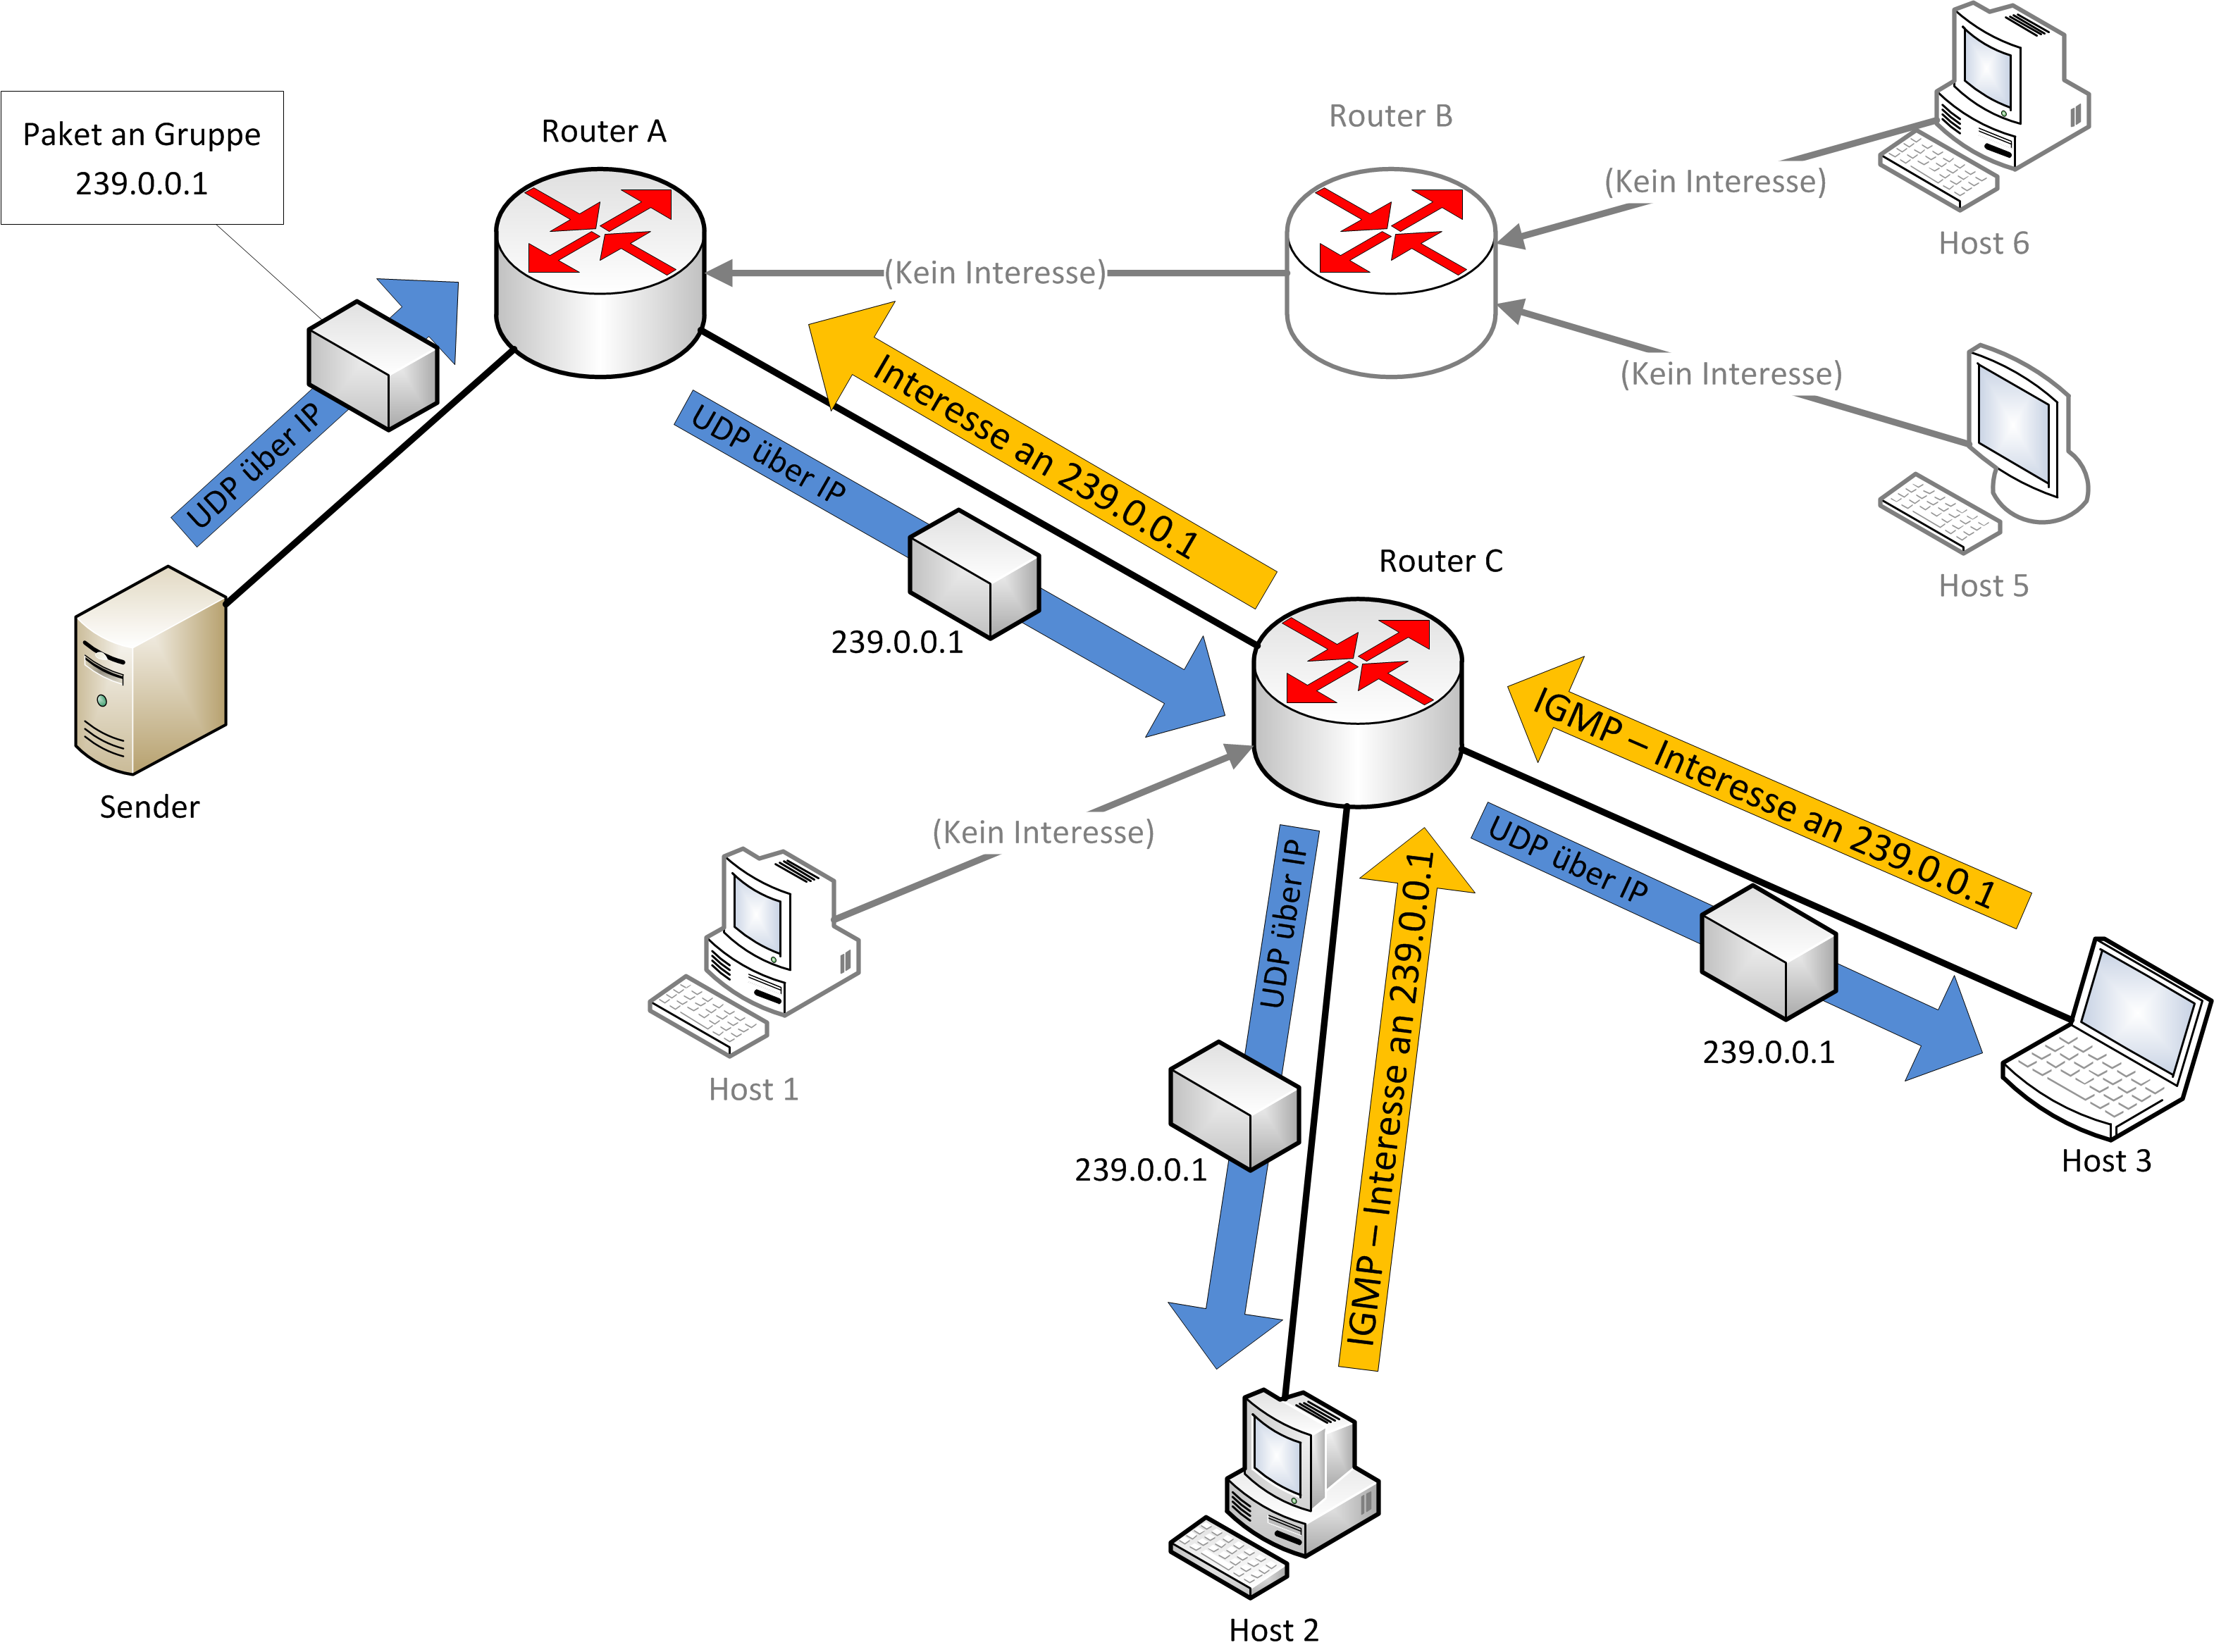
\includegraphics[width=15cm]{images/multicasting.png}
\centering
\caption{Schematische Verteilung eines Multicast-Pakets}
\label{mc_overview}
\end{figure}

Technisch wird Multicasting in OSI-Schicht 3 (Vermittlung/Network) bzw. der ihr
entsprechenden Internetschicht des TCP/IP-Referenzmodells umgesetzt.\\
\\
Wie oben erwähnt, wird Multicast-Datenverkehr durch Multicast-Gruppen und
dazugehörige IP-Adressen organisiert. Auf technischer Ebene heißt das, dass der
Sender in den IP-Header eines Datenpakets nicht die IP-Adresse eines bestimmten
Hosts, sondern eine Multicast-Adresse als Empfänger einträgt. Der
IP-Adressbereich von 224.0.0.0 bis 239.255.255.255 ist für
Multicast-Adressen reserviert (siehe hierfür z.B. RFC3171). Das so erzeugte
IP-Paket wird dann an den nächstgelegenen Router geschickt.\\
\\
Komplexe Multicast-Routing-Protokolle sorgen nun dafür, dass das Paket alle
Router, an die interessierte Hosts angeschlossen sind, erhalten. Um das Netzwerk
nicht unnötig zu belasten, sorgen sie auch dafür, dass Router, deren
angeschlossene Netzwerke überhaupt nicht am Multicast interessiert sind, die
Pakete auch nicht erhalten. Vor Allem muss aber vermieden werden, dass sich in
den Paket-Routen Zyklen bilden, da sie die Leistungsfähigkeit des Netzwerks
stark beeinträchtigen können. Auch wenn die Routing-Protokolle ebenfalls in
OSI-Schicht 3 agieren und \emph{Bestandteil} von IP sind, dienen sie selbst
\emph{nicht} der Datenübertragung. Sie dienen lediglich der Kommunikation der
Router untereinander, damit diese die Multicast-Pakete korrekt weiterleiten
können. Die Multicast-Pakete selber sind nach wie vor gewöhnliche IP-Pakete
(von der speziellen Empfängeradresse im Header abgesehen). Häufig verwendete
Multicast-Routing-Protokolle sind PIM, DVMRP (über IGMP, s.u.) und MOSPF.\\
\\
Um Multicast-Pakete zu empfangen, muss sich ein Host bei einer Multicast-Gruppe
anmelden. Er teilt dazu dem Router, an den er angeschlossen ist mit, dass er an
einer bestimmten Multicast-Gruppe interessiert ist. Die gewünschte
Multicast-Gruppe wird durch ihre Multicast-IP-Adresse spezifiziert. Der Router
weiß nun, dass der angeschlossene Host an allen Paketen interessiert ist, die
diese Multicast-Adresse im Empfängerfeld tragen. Der Host teilt dem Router sein
Interesse über das \emph{Internet Group Management Protocol (IGMP)} mit. Wie
die Routing-Protokolle ist auch dieses Protokoll wieder Teil von IP, dient aber
ebenfalls nicht der Datenübertragung selbst, sondern nur der Kommunikation der Netzwerkknoten
untereinander. Tatsächlich verwendet auch das oben erwähnte DVMRP zum
Informationsaustausch IGMP-Pakete.\\
\\
Das Versenden und Empfangen eines Multicast-Pakets, sowie die dazu
notwendige Interaktion der beteiligten Netzwerkkomponenten ist in Abbildung
\ref{mc_overview} schematisch dargestellt.

\subsection{Multicasting unter Java}

Die zum Einsatz kommende Java Platform Standard Edition 6 stellt für
Multicast-Anwendungen die \emph{MulticastSocket}-Klasse zur Verfügung. Der
MulticastSocket stellt Methoden zum transparenten Senden und Empfangen von
UDP-Multicast-Paketen bereit. Von der Anwendung werden zum Senden der
Paketinhalt und die Ziel-Gruppenadresse übergeben. Analog wird zum
Empfangen eines Multicast-Streams die gewünschte Gruppenadresse übergeben. Alle
übrigen zur Kommunikation benötigten Systemaufrufe und Mechanismen werden von
der Klasse verborgen. Eine gesonderte Auseinandersetzung mit IGMP oder
Multicast-Routing ist daher auf Anwendungsebene nicht mehr nötig. Aus Sicht des
OSI- und auch des TCP/IP-Schichtenmodells stellt ein Socket damit die Verbindung
zur Transportschicht (OSI-Layer 4) her.

\subsection{Einordnung des Tools}

\begin{figure}[H]
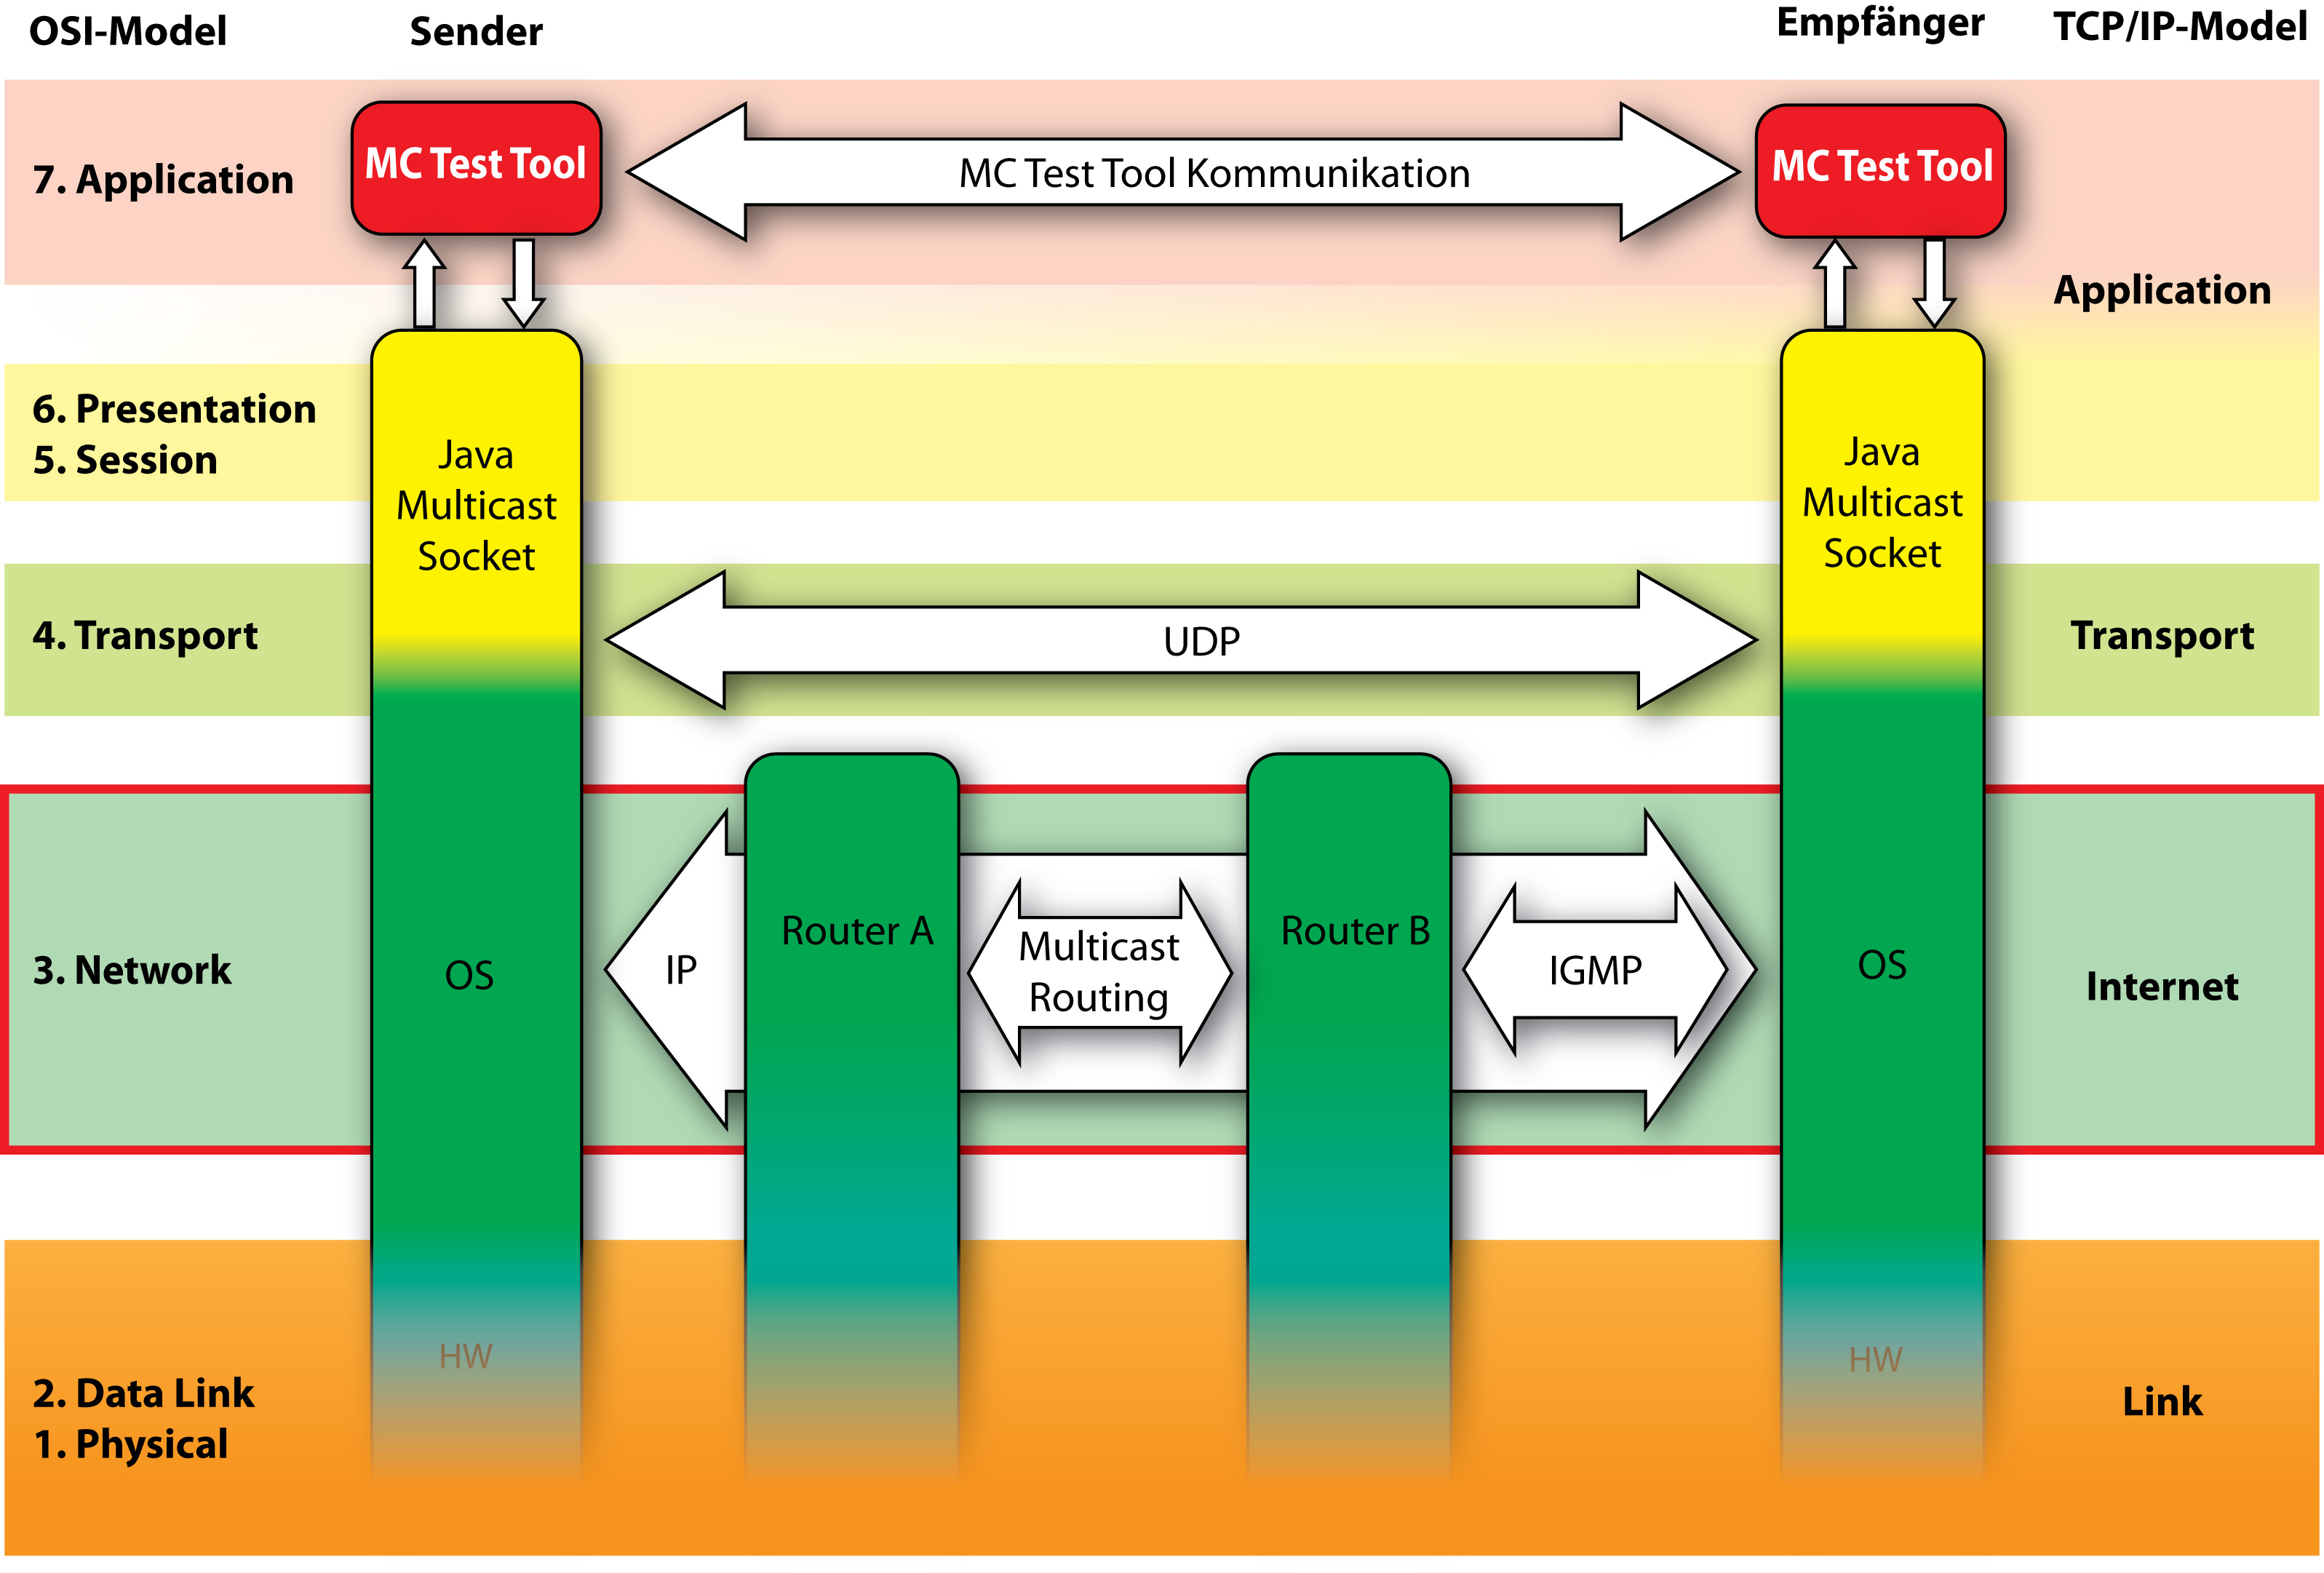
\includegraphics[width=15cm]{images/mc_osi_einordnung.jpg}
\centering
\caption{Einordnung des Gesamtsystems in das OSI- bzw. TCP/IP-Schichtenmodell}
\label{mc_osi_einordnung}
\end{figure}

Hauptaufgabe des Multicast Test Tools ist es, wie bereits beschrieben, die
Multicasting-Fähigkeiten eines Netzwerkes zu testen. Seine Analysen
konzentrieren sich also vor Allem auf die Netzwerkschicht (Schicht 3) des
OSI-Modells bzw. die Internetschicht des TCP/IP-Modells. Den Zugriff auf diese
Schicht stellt der MulticastSocket der Java Platform zur Verfügung. Obwohl also
die Netzwerkschicht Ziel der Untersuchungen ist, wird sich der tatsächliche
Programmieraufwand fast ausschließlich auf die Anwendungsschicht (OSI 7)
konzentrieren.\\
Die Abbildung gibt einen Überblick über die Einordnung des
Systems ins OSI- bzw. TCP/IP-Modell.

\section{Systemanalyse}
%Analyse der Rahmenbedingungen 
%Analyse der Problemstellung 
%Architektur und Gliederung der Komponente 
%Interaktionsanalyse / Abhängigkeiten 
%Weitere Dekomposition 

\subsection{Einordnung in das Gesamtsystem}

%Hier erstmal kurz beschreiben was die Probleme sind. Noch nicht die Lösung.

Durch die relativ hohe Komplexität des Gesamtsystems, müssen Techniken angewendet werden um diese Komplexität herunterzubrechen und dadurch handhabbar zu machen. Zudem sollten Abhängigkeiten zwischen Modulen, so gut wie möglich, vermieden werden. Auch die 
Implementierung einzelner Module, sollte für andere Komponenten des Systems keine Rollen spielen.
\\
Dieses Modul ist im Model der Applikation angesiedelt.
Dort wird es von dem Modul verwendet, das sich um das versenden der Pakete über das Netzwerk kümmert.
Abhängigkeiten von anderen Modulen des Systems gibt es keine.
\\
Das Modul wird von einer stark parallelisierten Komponente verwendet. Aus diesem Grund muss das Modul robust gegen die Probleme von Nebenläufigkeit entworfen werden.

\subsection{Gliederung des Moduls}
\label{sec:7:speed}
Zehntausende von Paketen pro Sekunde zu Verarbeiten kann sehr kritisch für die Performance des Gesamtsystems sein.
Aus diesem Grund sind bei allen Überlegungen zum Design des Moduls auch immer die Auswirkung auf die Performance zu betrachten.
Ein weiterer wichtiger Aspekt des internen Designs des Moduls ist die Erweiterbarkeit um neue Paketformate.
Wie wir wissen werden etliche Konkurrenzprodukte parallel entwickelt. So kann es in der Zukunft durchaus nötig
werden das Tool um Kompatibilität mit anderen Tools zu erweitern. Zudem muss, durch die Kompatibilität zum Hirschmanntool, schon
ein gewisses Maß an Transparenz zum verwendeten Paketformat gegeben sein.

\subsection{Kompatibilität zum Hirschmann Tool}
\label{sec:7:comaptability}

Um die Kompatibilität zum Hirschmann Tool zu wahren, müssen Hirschmann Pakete sowohl geparsed als auch erstellt werden.
Welches Paketformat verwendet wird, sollte für den Benutzer dieses Moduls möglichst transparent sein. Da das Hirschmann Paketformat nicht spezifiziert ist, müssen
Methoden des Reverse Engineering angewendet werden. Hierzu stehen sowohl der Originalsourcecode, zum Erstellen des Pakets in der Programmiersprache C, sowie mit Wireshark abgefangene Pakete zur Verfügung.

\subsection{Problemstellung und Anforderungen}

Wie in der SRS spezifiziert, muss die Applikation einige Anforderungen erfüllen.
Die für dieses Modul relevanten Anforderungen sind:

\paragraph{Performance}
Beim gleichzeitigen Betrieb von 30 Datenströmen dürfen
bei einem handelsüblichen Rechner mit 2,4GHz Intel Core 2 Duo Prozessor und 2GB RAM nicht mehr als 80\%
des Systems ausgelastet werden.

\paragraph{Effizienz} Das Programm stellt die geforderte Funktionalität durch
lineare und direkte Datenverarbeitungswege ohne unverhältsnismäßig hohe
Rechnerbelastung zur Verfügung. Zur Verhältnismäßigkeit muss beachtet werden,
dass das Senden und Empfangen von vielen Datenströmen speziell mit hohen
Frequenzen durchaus viel Rechenleistung erfordern kann.

\paragraph{Verteilung, Kommunikation mit anderen Systemen, Migration}
Mehrere, voneinander funktional-unabhängige Instanzen des Systems können auf
vielen verschiedenen Knoten eines Netzwerks in Betrieb genommen werden können. Diese
kommunizieren dabei untereinander oder mit dem alten
System der Hirschmann Automation GmbH.

\paragraph{Parallelisierung}
Die einzelnen Datenströme werden mit den Mitteln der Java-Plattform
parallelisiert. Die Java-Virtual-Machine entscheidet weiterführend, wie die
Parallelisierung auf Rechner-Ebene umgesetzt wird.

\paragraph{Stabilität} Die Architektur beachtet die Tatsache, dass in einem
offenen Netzwerk nicht nur wohlgeformte Pakete an den Empfänger gelangen können.
Das Paket-Dekodierungs System wird diese, nicht dem Protokoll
entsprechenden Pakete erkennen und verwerfen ohne das es zu Fehlern im System
kommt.

\paragraph{Wartbarkeit} Jeder Teil der Architektur strebt hohe
Kohäsion und geringe Kopplung an. Somit sind alle wichtigen Komponenten
individuell austausch- und testbar. Durch häufige Verwendung des
Beobachter-Entwurfsmusters wird eine sehr einfache Erweiterbarkeit des Systems
ermöglicht.

\paragraph{Portabilität} Um das Tool auf allen großen Plattformen verfügbar zu
machen, wird als Implementierungssprache Java in der Version 6 gewählt. Das Tool
basiert komplett auf der Java API sowie Java-nativen, externen Bibliotheken.
Dadurch müssen keine Plattform-spezifischen Anpassungen durchgeführt werden.

% ==============================================================================
%
% DESIGN
%
% ==============================================================================

\chapter{Design}
%Folgerungen aus der Analyse 
%Lösungen für den Problembereich der Analyse 
%Systemarchitektur 
%Anwendung der Basiskonzepte des Softwareengineerings
%Schnittstellen

\section{Systemarchitektur}
\label{sec:7:sysarch}

Das Gesamtsystem wird zur besseren Verständlichkeit und zur Vermeidung von Abhängigkeiten 
in logische Komponenten unterteilt. Dabei ist das Gesamtsystem zeitgemäß auf höchster Abstraktionsebene nach dem Model-View-Controller-Entwursmuster entworfen. Dieses Pattern gliedert die Applikation in drei Untermodule, das Model, die View und den Controller.
Dabei werden Programmlogik (Model) und Darstellung (View) voneinander
entkoppelt und kommunizieren über eine Steuerschicht (Controller) miteinander.
So herrscht zwischen den einzelnen Komponenten eine strenge Hierarchie. Das Model weiß von keinem Controller und
der Controller kennt keine View. Durch diese Trennung besteht eine sehr schwache Kopplung zwischen den einzelnen
Komponenten. Diese Flexibilität ist ausschlaggebend für die Anpassungsfähigkeit der Applikation an ein sich änderndes Umfeld. 

\begin{figure}[H]
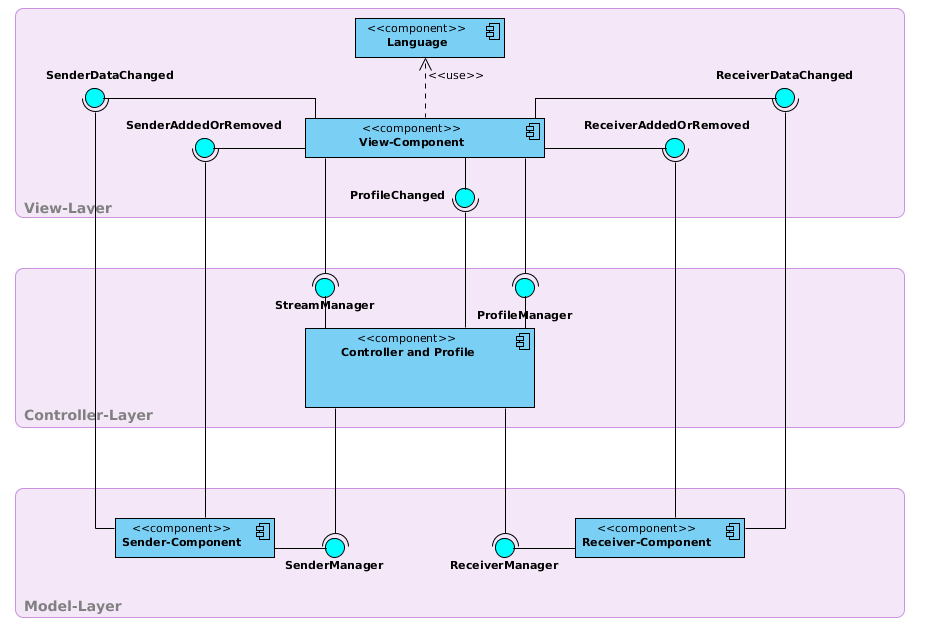
\includegraphics[width=15cm]{images/Overview.png}
\centering
\caption{Komponentendiagramm: Gesamtsystem}
\label{uml_controller}
\end{figure}

Wegen der relativ hohen Komplexität der einzelnen Komponenten, des Model-View-Controller Patterns, werden diese, bei Bedarf und wenn es sich anbietet, noch in kleinere Subkomponenten unterteilt. Auch beim Model ist dies der Fall. Eines dieser Subkomponenten ist die Paket Komponente die in dieser Moduldokumentation beschrieben ist.
\\
In der folgenden Abbildung ist die Beziehung der Paket Komponente zu den Klassen der Netzwerk Komponente zu sehen.
Wie man sieht ist das Interface zu der Umgebung sehr klar abgegrenzt und ohne zirkuläre Abhängigkeiten.

\begin{figure}[H]
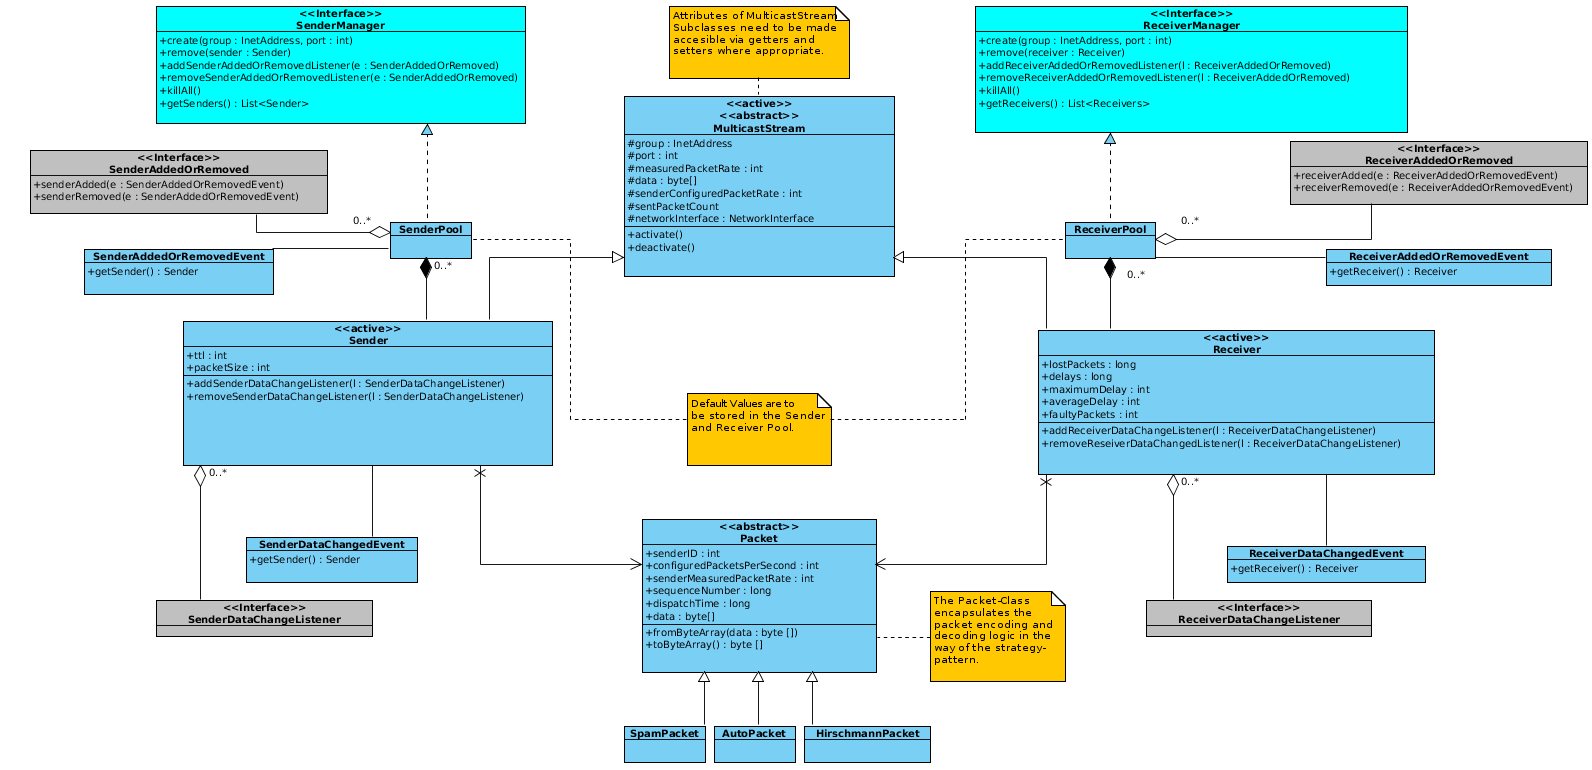
\includegraphics[width=15cm]{images/Model.png}
\centering
\caption{Klassendiagramm: Model}
\label{uml_controller}
\end{figure}

% ===============================
%
% MODUL DESIGN
%
% ===============================


\section{Interface Design}
\label{sec:7:packet}

Wie schon im Abschnitt zur Systemarchitektur erwähnt, wurde durch die Umsetzung eines klaren und einfachen Interfaces, sehr viel Wert auf die Abgrenzung der Komplexität dieses Moduls zu seinem Umfeld gelegt. Auch die Vermeidung von zyklischen Abhängigkeiten zu anderen Modulen konnte komplett vermieden werden. Die Definition dieses Interfaces ist im folgenden UML Diagramm zu sehen.

\label{sec:4:empf}
\begin{figure}[H]
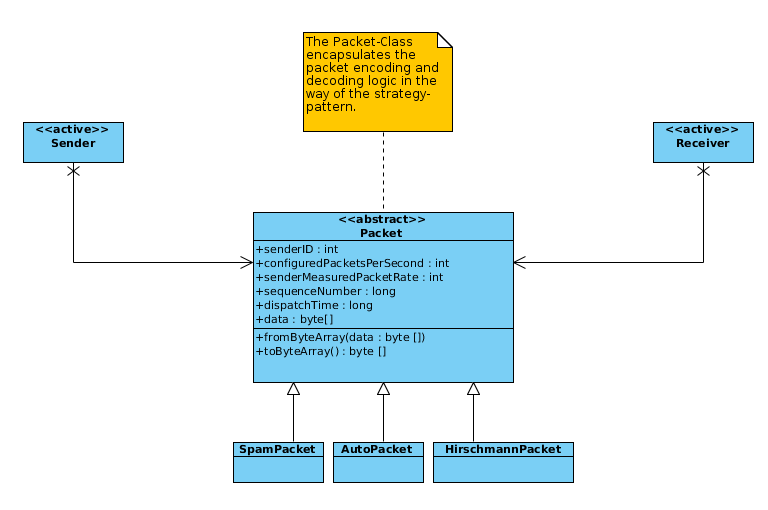
\includegraphics[width=15cm]{images/Package.png}
\centering
\caption{Klassendiagramm: Paketkomponente}
\label{uml_controller}
\end{figure}

Es ist anzumerken, dass alle public declarierten Felder durch Setter und Getter implementiert wurden.
Detailiertere Beschreibungen der Interfaces und Klassen sind in der Javadoc zu finden.
\\\\
Um die relevanten Daten aus den UDP Paketen zu extrahieren, wird ein Strategy Pattern verwendet.
Dieses Pattern, verbirgt den Algorithmus zum Parsen des Pakets aus dem UDP Bitstream, hinter einem von der
Implementierung unabhängigen Interface. Folglich ist das verwendete Paketformat für 
den Benutzer des Interfaces vollkommen transparent.
\\\\
In der folgenden Abbildung wird beschrieben wie ein Multicast Paket empfangen und
dann in ein Objekt umgewandelt wird. Es zeigt anschaulich den dynamischen Verlauf des Empfangs eines Pakets.

\begin{figure}[H]
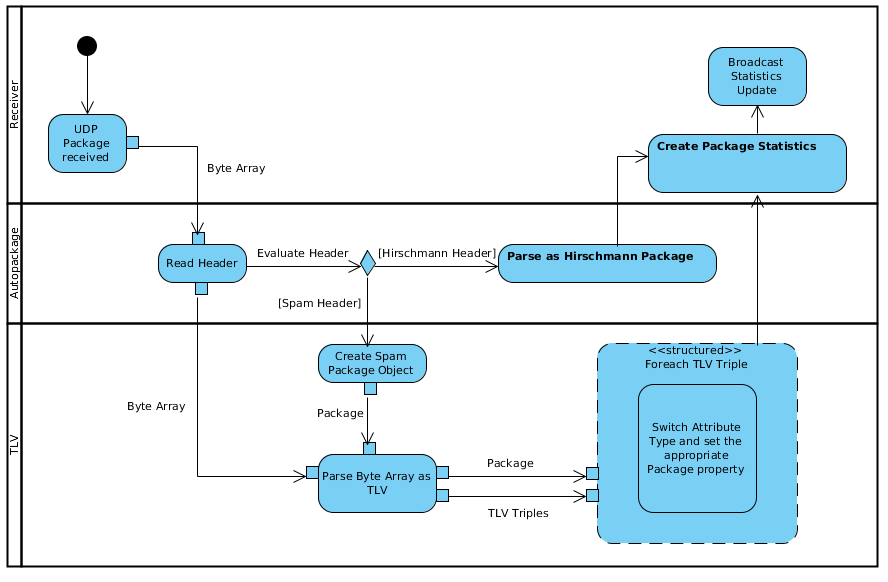
\includegraphics[width=15cm]{images/Receive.png}
\centering
\caption{Empfang eines Mutlicast-Pakets - UML Activity Diagramm}
\label{fig_receive}
\end{figure}


\section{Autopacket Klassen Design}

Diese Klasse erkennt automatisch, am Header eines Pakets, welche Art von Parser 
verwendet werden muss. Hierdurch wird der Benutzer des Interfaces komplett 
vom Verständnis diesem Detail der Implementierung befreit.

\section{SPAM Klassen Design}
\label{sec:7:packet}

Um das Parsen des Pakets zu vereinfachen, wird auf die einheitliche Struktur des TLV Formats zurückgegriffen.
Jedes konkrete TLV Tupel (wie zum Beispiel die SenderId), implementiert ein Interface um die Daten eines TLV
Tupels zu verarbeiten oder zu schreiben. Durch die Anwendung dieses Strategy Pattern, lässt sich der
Parser des SPAM Paketformats sehr einfach erweitern.
\\
\\
Die häufige Verwendung des Strategy Pattern hat nicht nur den Vorteil der einfacheren Erweiterbarkeit. Durch das Auslagerung von Logik in eine eigene Klasse, können Programmfehler, durch inkonsistente Änderungen an Code Duplikaten, vermieden werden. 
\\
\\
Wie schon erwähnt, ist es immer wichtig auch die Geschwindigkeitseinbusen eines schönen Designs zu beachten.
Die hier verwendeten Strategien, können relativ gut von einem Just In Time Compiler Optimiert werden.
Wegen der Geschwindigkeitseinbusen konnte ein Design mit Reflektion, und der damit
verbundenen Vereinfachung des Codes, nicht umgesetzt werden.

\section{SPAM Paket Protokoll}

Um die Testbarkeit eines Multicast Netzwerkes zu ermöglichen, muss das Tool notwendigerweise
Datenpakete via Multicast versenden können. Die versendeten Pakete müssen Informationen über den
Zustand der Applikation zum Zeitpunkt des Versands beinhalten, um so beim Empfänger
Statistiken über die Übertragung erstellen zu können. Um die nötigen Informationen
zu strukturieren ist ein Datenformat von Nöten. Die Struktur sollte einfach
Erweiterbar und trotzdem simpel gehalten sein um das Dekodieren der Pakete 
effizient zu gestalten. Das TLV Protokoll erfüllt all diese Anforderungen.
TLV steht für Type-Length-Value-Format und wird in vielen vorhandenen 
Netzwerkprotokollen, wie zum Beispiel COPS, IS-IS, LLDP und RADIUS genutzt,
wobei es sich dort als erweiterbar und robust bewährt hat.
Bei diesem Protokoll wird jedes Attribut eines Paketes durch folgendes Tripel übermittelt:

\begin{itemize}
 \item[-] Type: bestimmt den Typ des Attributes, in unserem Fall ein unsinged 
                16bit Integer.
 \item[-] Length: bestimmt die Länge des Attribut Wertes und ist 
                  in unserem Fall ein unsigned 32bit Integer.
 \item[-] Value: enthält den eigentlichen Wert des Attributes.
\end{itemize}

Durch die einheitliche Struktur des Protokolls ist es sehr einfach Sequenzen von
TLV Tripel mit einer einheitlichen Funktion zu durchsuchen.
Hierbei werden Tripel mit einem unbekannten Typen ignoriert, was zu einer 
einfachen Erweiterbarkeit führt. Die Anzahl der Tripel im Paket muss nicht 
angegeben werden, da die Länge des Paketes schon im UDP Header enthalten ist.
Zudem kümmert sich UDP auch um die Integrität der Daten, ein extra CRC Hash oder
Paritybits müssen also nicht mit übertragen werden. Alle Datenfelder werden
im Big Endian Format representiert.
\\ \\
Um das hier spezifizierte Protokoll vom Hirschmann-Protokoll und anderen
Protokollen zu unterscheiden, ist ein Header vor den TLV Attributen wichtig. Daher muss vor dem ersten TLV Trippel 
folgendes Hexadezimales Bytemuster stehen.
\\ \\
05 39 00 00 00 00
\\ \\
Diesen Header kann man auch als TLV Trippel mit dem Typ 1337, der Datenlänge
0 und keinen Nutzdaten auffassen. Dieser Umstand vereinfacht potentiell das parsen des Protokolls.
\\ \\
\textbf{Das Protokoll kann wie folgt als DD dargestellt werden:} \\ \\
Paket = Header + {TLV} \\
Header = 0x053900000000 \\
TLV = Type + Length + Value  \\
Type = 0..65535  \\
Length = 0..4294967295 \\
Value = Datenstrom der zuvor genannten Länge. \\
\\ 
\begin{table}[htdp]
\centering
\caption{Im Protokoll verwendete Attribute}
\label{tab:prot}
\begin{tabular}{|l|l|p{9.5cm}|}
\hline
\textbf{Beschreibung} & \textbf{Typ} & \textbf{Attribut Wert} \\
\hline
Sender ID & 1 & Signed 32bit Integer Sender ID.\\
\hline
Eingestellte Paketsenderate & 2 & Pakete pro Sekunde als unsigned 32 bit Integer. \\
\hline
Ermittelte Paketsenderate & 3 & Pakete pro Sekunde als unsigned 32 bit Integer. \\
\hline
Sequenznumber & 4 & Signed 32bit Integer Sequenznumber. \\
\hline
Absendezeit & 5 & Nanosekunden seit dem 1. Januar 1970 00:00 Uhr UTC (vergleiche Unixzeit) als signed 64 bit Integer. \\
\hline
Daten & 6 & Datenstream variabler Länge. \\
\hline
Padding & 7 & Feld zum Auffüllen des Pakets auf eine bestimmte Länge. \\
\hline
\end{tabular}
\end{table}

\chapter{Implementierung}
%Vorgehen 
%Zwischenergebnisse 
%Anwendung der Basiskonzepte 
%Codedokumentation 

\section{Umsetzung von Anforderungen}
In diesem Abschnitt wird beschrieben, wie die Anforderungen der Analyse umgesetzt wurden.

\paragraph{Performance}
Die nötige Performance wurde durch den Verzicht auf übertriebene architektonische 
Schönheit und die Verwendung von Javas Lowlevel Funktionalitäten erreicht.

\paragraph{Verteilung, Kommunikation mit anderen Systemen, Migration}
Die Kommunikation mit dem alten
System der Hirschmann Automation GmbH wird durch eine Komponente erreicht, die sowohl Hirschmann Pakete parsen wie auch erstellen kann.

\paragraph{Parallelisierung}
Um das Modul in einer parallelen Umgebung zu verwenden, darf ein Paket Objekt nicht
zwischen mehreren Threads ausgetauscht werden. Dies bedeutet, dass für das Parsen und 
Erstellen eines Pakets immer ein neues Packet Objekt erstellt werden sollte.
Diese Restriktion sollte in der Praxis kein Problem darstellen.
Die Möglichkeit der Parallelisierung wird durch den kompletten Verzicht von schreibenden Zugriffen auf statische Variablen erreicht.

\paragraph{Stabilität} Einkommende Pakete werden sehr sorgfältig geparsed.
Sind Felder fehlerhaft, so werden die Pakete verworfen. Auch wenn sehr große 
TLV Tupel angegeben werden, wird nicht einfach blind Speicher angefordert. Hierdurch
werden Denial Of Service Angriffe vermieden.

\paragraph{Wartbarkeit} Das Paket strebt hohe
Kohäsion und geringe Kopplung an. Somit sind alle wichtigen Komponenten
individuell austausch- und testbar. Durch Verwendung des Strategy Pattern ist eine einfache Erweiterbarkeit des Systems
ermöglicht.

\paragraph{Portabilität} Es wird Java verwendet und auf Portabilität zum Beispiel
bei Endianness geachtet.

\section{Hirschmann Paket Checksummen Algorithmus}

Das Hirschmann Paketformat verwendet einen nicht standardisierten Checksummen Algorithmus 
um Pakete auf Übertragungsfehler zu überprüfen. 
Die Checksumme könnte auf der Empfangsseite theoretisch einfach ignoriert werden. Will man allerdings
Pakete an die Originalanwendung schicken, so muss die Checksumme richtig berechnet werden. Wäre sie falsch,
würde das Paket einfach von Empfänger abgelehnt, wodurch eine sinnvolle Kommunikation
unmöglich wäre.
\\
\\
Es ist noch zu erwähnen, dass solch eine Checksumme völlig überflüssig ist. 
Wäre beim Design dieses Protokolls eine gründliche Analyse des Multicast Standards vorgenommen worden, so wie dies in den Voruntersuchungen zu diesem Protokoll gemacht wurde, wäre dem Entwickler aufgefallen, dass die 
Integrität eines UDP Pakets schon vom UDP Standard selbst überprüft wird.
\\\\
Wie dem auch sei, im folgenden soll der verwendete Checksummen Algorithmus diskutiert werden.

\newpage
\begin{lstlisting}

UINT16 CIP_Multicast_SenderDlg::UdpDataCalcCheckSum(UINT16 *addr, UINT16 len, UINT16 csum) {
    register UINT32 nleft = len;
    const UINT16 *w = addr;
    register UINT16 answer;
    register UINT32 sum = csum;

    /*  Our algorithm is simple, using a 32 bit accumulator (sum),
     *  we add sequential 16 bit words to it, and at the end, fold
     *  back all the carry bits from the top 16 bits into the lower
     *  16 bits.
     */
    while (nleft > 1) {
        sum += *w++;
        nleft -= 2;
    }

    if (nleft == 1)
        sum += htons(*(UINT8 *) w << 8);
    // sum += hmApiOsHtons(*(hm_uchar8 *)w << 8);

    sum = (sum >> 16) + (sum & 0xffff); /* add hi 16 to low 16 */
    sum += (sum >> 16); /* add carry */
    answer = (UINT16) (~sum); /* truncate to 16 bits */
    // answer = (hm_uint16)(~sum);  
    return (answer);
}
\end{lstlisting}

Diesen Code nach Java zu übersetzen ist prinzipiell kein Problem. Java stellt
genau die gleichen Operatoren bereit und auch die hier verwendeten Typen haben, wie in Java,
eine fixe und platformunabhängige Anzahl von Bits. Allerdings gibt es in Java keine
unsigned Typen wie sie hier verwendet werden. Um dieses Problem zu umgehen, müssen
einige Variablen, vor ihrer Verwendung, vom Typ erweitert werden. Ein Short muss also
zum Beispiel in einen Integer umgewandelt werden. Damit dabei das Bitmuster gleich bleibt 
verwendet man den Trick einer binären Verundung.

\begin{lstlisting}
short a;
int b = b & 0xFFFF;
\end{lstlisting}

Auch die Parameter der Funktion müssen angepasst werden. Statt der Kombination aus Array Pointer und Array Länge
wird ein ByteBuffer aus der Java Standardbibliothek verwendet. Das order Argument
kann vorerst ignoriert werden. Später wird darauf noch eingegangen.
\\\\
Der htons Funktionsaufruf ist wohl der komplizierteste Teil des Algorithmus.
Zuerst wird der Parameter der Funktion vorbereitet. Dazu wird das aktuelle Byte in w gelesen.
Dieses sei zum Beispiel
\\
\\
0x5A
\\
\\
dann wird es um ein Byte geshiftet. Das Ergebnis ist
\\
\\
0x5A00
\\
\\
Daraufhin wird die Funktion htons aufgerufen. Diese ändert die Byteorder des Parameters 
von der des Systems in die Netzwerk Byteorder. Die Netzwerk Byteorder ist immer Big Endian.
Da das Programm wohl auf einem Intel Computer entwickelt wurde (Little Endian) werden
die Bytes also umgedreht. 
\\
\\
5A
\\
\\
Der ganze Aufwand war also umsonst und kann weggelassen werden. Hier die 
Implementierung des Codes in Java.

\newpage
\begin{lstlisting}
private static short generateChecksum(ByteBuffer data, ByteOrder order) {
    long sum = 0;
   
    data.order(order);
   
    // Our algorithm is simple, using a 32 bit accumulator (sum),
    // we add sequential 16 bit words to it, and at the end, fold
    // back all the carry bits from the top 16 bits into the lower
    // 16 bits
    while (data.remaining() > 1) {
        int c = data.getShort() & 0xFFFF;
        sum += c;       
    }
   
    // if buffer can't be split in shorts
    // imagine appending 0x00 to the buffer
    if (data.limit() % 2 == 1) {
        sum += (data.get(data.limit()-1) & 0xFF);
    }
           
    // add hi 16 to low 16
    sum = (sum >> 16) + (sum & 0xFFFF);
    // add carry
    sum += (sum >> 16);                
   
    // truncate to 16 bits
    return (short)(~sum);
}
\end{lstlisting}

Wie versprochen, wird jetzt noch auf den order Parameter eingegangen.
Die C Implementierung des Algorithmus wird wie folgt aufgerufen.
\begin{lstlisting}
UdpOperData_t myThreadUdpOperDataBuffer; // without big endian
checksumBuffer = (char*) & myThreadUdpOperDataBuffer;
myThreadUdpOperDataBuffer.Checksum = 
    CIP_Multicast_SenderDlgBuffer.UdpDataCalcCheckSum(
        (UINT16*) checksumBuffer, sizeof (myThreadUdpOperDataBuffer), 0); 
\end{lstlisting}

Aus Wireshark Mitschnitten, konnte Reverse Engineered werden, dass das Protokoll für die Übertragenen Daten Netzwerk Byteorder,
also Big Endian verwendet. Wie man sieht, wird die Checksumme aber nicht auf dem versendeten Paket, sondern auf
einer Struktur berechnet. Diese hat naturgemäß die Byteorder des verwendeten Systems.
Folglich werden Anwendung die auf zwei verschiedenen Architekturen laufen nicht miteinander kommunizieren können.
\\\\
Um trotzdem empfangskompatibel zu sein, werden beim Empfangen die Checksummen sowohl für ein Big Endian
als auch für ein Little Endian Paket überprüft. Dies erklärt auch warum ein
order Parameter an die Checksummen Funktion übergeben wird. Er gibt an ob die Checksumme
für Little oder Big Endian generiert werden soll. 
Da das Empfangene Paket in jedem Fall als Big Endian vorhanden ist, muss bei der Überprüfung das Paket auch noch
im Little Endian Format neu generiert werden.
\\\\
Beim Senden können wir allerdings nicht wissen was für eine Architektur der Empfänger verwendet und daher müssen wir hier raten. Da wohl die meisten CPUs von Intel sind, werden standardmäßig Little Endian Checksummen generiert.
\\\\
Folgender Kommentar zeigt, dass der Designer der Spezifikation sogar wusste was er macht. Das Design ist also nicht durch Dummheit, sondern nur durch den Drang zur Folter späterer Programmierer zu erklären. 
\begin{lstlisting}
// without big endian
\end{lstlisting}

Folgend noch der Sourcecode zum Empfangen von Paketen. Hier ist der zuvor beschriebene Mechanismus zum Überprüfen der Checksumme zu sehen.

\newpage
\begin{lstlisting}
public void fromByteArray(ByteBuffer data) throws DataFormatException
{
    minSize = 0;
    senderID = 0;
    configuredPacketsPerSeconds = 0;
    sequenceNumber = 0;
   
    try {
        data.order(ByteOrder.BIG_ENDIAN);
       
        // create data buffer to check for big endian checksums
        ByteBuffer bigEndianCheckData = data.duplicate();
        bigEndianCheckData.limit(CONSTSIZE-2);
       
        // skip header
        data.position(data.position()+HEADER.length);
       
        // read fields
        setSenderId(data.getShort() & 0xFFFF);
        setSequenceNumber(data.getInt() & 0xFFFFFFFFL);
        setConfiguredPacketsPerSecond(data.getShort() & 0xFFFF);
        short ttl = (short)(data.get() & 0xFF);
        long reset = data.getInt() & 0xFFFFFFFFL;
        short check = data.getShort();
       
        // regenerate the packet as little endian
        ByteBuffer checkData = createUncheckedByteArray(ttl,reset,ByteOrder.LITTLE_ENDIAN);
        // check both little and big endian checksum
        if(generateChecksum(checkData,ByteOrder.LITTLE_ENDIAN) != check) {
            if(generateChecksum(bigEndianCheckData,ByteOrder.BIG_ENDIAN) != check) {
                throw new DataFormatException("Invalid checksum");
            }
        }
    } catch(BufferUnderflowException e) {
        throw new DataFormatException("Illegal Hirschmann Package Format");
    }
}
\end{lstlisting}


\chapter{Komponententest}
%Wie wird die Komponente getestet? 
%Dokumentation von Vorgehen und Ergebnissen. Bei Bedarf entsprechend erweitern

Da die komplette Applikation auf dem Code dieses Moduls aufbaut, ist es extrem wichtig die
Komponente richtig zu testen. Wenn Benutzer dieses Interfaces Fehler komplett ausschließen können, erleichtert sich 
die Programmierung ihrer Komponenten enorm. 

Die korrekte Funktionalität des Paket Moduls wird hauptsächlich über Junit-Tests, sowie
System-Tests realisiert. Die zugehörigen Testsuiten finden sich in dem STP, die zuge-
hörigen Ergebnisse in dem STR. Die Systemtests bzw. deren Ergebnisse werden hier
aufgrund von Redundanz nicht erneut hinterlegt.
Die betreffenden Testsuiten lauten:
\begin{enumerate}
\item /UC30/ Fehlerfreier Austausch von MC Paketen
\item /UC40/ Analyse und Anzeige von Messdaten 
\end{enumerate}

Die Testsuiten testen im Prinzip, sowohl die korrekte Übertragung von Feldern in Paketen, sowie die
Möglichkeit überhaupt Pakete so zu verschicken.
Viele Tests können aber auch automatisiert werden, da das Parsen von Paketen 
recht einfach direkt über einen Komponententest erfolgen kann.
Die Tests werden automatisiert von unserem Continuous Integration Environment ausgeführt und ermöglichen somit eine stetige Überprüfung der korrekten Funktionalität der entsprechenden
Komponente. Alle automatisierten JUnit Tests befinden
sich in „src/test/java/com/spam/mctool/model/packet“. 

\newpage

\section{Komponententestplan}

\begin{table}[h]
\caption{Komponententestplan}
\label{tab:ktp}
\begin{center}
\begin{tabular}{|p{2cm}|p{6cm}|p{6cm}|}
\hline
\textbf{Test Nr.} & \textbf{Test Methode} & \textbf{Beschreibung}\\
\hline
/CTC0601/ & testValidHirschmannPackets & Testet das Erstellen und Parsen valider Hirschmann Pakete\\
\hline
/CTC0602/ & testInvalidHirschmannPackets & Testet das Erstellen und Parsen invalider Hirschmann Pakete\\
\hline
/CTC0603/ & testValidSpamPackets & Testet das Erstellen und Parsen valider SPAM Pakete\\
\hline
/CTC0604/ & testInvalidSpamPackets & Testet das Erstellen und Parsen invalider SPAM Pakete\\
\hline
/CTC0605/ & testPackagePadding & Testet das Padding eines Pakets\\
\hline
/CTC0606/ & testIllegalArguments & Testet die Verwendung des Packet Interface mit invaliden Werten\\
\hline
\end{tabular}
\end{center}
\end{table}

Folgend eine Beschreibung der einzelnen automatisierten Tests

\subsection{/CTC0601/} 
Testet das Erstellen und Parsen valider Hirschmann Pakete. Das Testpaket ist wie folgt binär aufgebaut
und wurde bei mit Wireshark aus dem Outputstream des Originaltools mitgeschnitten.
\\\\
Hirschmann IP Test-Multicast 0x00   \\
0x7E 0xCD                           \\
0x00 0x00 0x00 0xE6                \\
0x00 0x01                           \\
0x20                                 \\
0x00 0x00 0x00 0x00                  \\
0xDA 0x5F                            \\
\\\\
Während des Tests wird dieser Bytestream zuerst in eine Paket Klasse umgewandelt.
Aus diesem Paket wird dann wieder ein Bytestream generiert. Der resultierende Bytestream
wird erneut geparsed und es wird überprüft ob alle Wert immer noch korrekt sind.

\subsection{/CTC0602/} 
Test
et das Erstellen und Parsen invalider Hirschmann Pakete. Das Testpaket ist wie folgt binär aufgebaut.
\\\\
Hirschmann IP Test-Multicast 0x00   \\
0x7E 0xCD                           \\
0x00 0x00 0x00 0xE6 \\
0x00 0x01                                \\
0x20                      \\                   
0x00 0x00 0x00 0x00     \\
0xDA 0x5F\\
0xFF                    
\\\\ 
Während des Tests wird dieser Bytestream zuerst in eine Paket Klasse umgewandelt.
Auftretende Fehler werden abgefangen und ausgewertet. In mehreren weiteren Tests
werden einige Byte des Pakets verändert und Fehler werden erneut abgefangen und ausgewertet.

\newpage

\subsection{/CTC0603/} 
Testet das Erstellen und Parsen valider SPAM Pakete. Das Testpaket ist wie folgt binär aufgebaut.
\\\\
5 57  0 0 0 0                       \\         
0 1   0 0 0 4     -1  -1  -1  -1       \\
0 2   0 0 0 4    127  -1  -1  -1           \\
0 3   0 0 0 4      5 127   0 111           \\
0 4   0 0 0 4     -1  -1  -1  -1           \\
0 99  0 0 0 9    IGNORE ME    \\
0 5   0 0 0 8     -1  -1  -1  -1  -1  -1  -1  -1    \\
0 6   0 0 0 4    Test     \\\\
Während des Tests wird dieser Bytestream zuerst in eine Paket Klasse umgewandelt.
Aus diesem Paket wird dann wieder ein Bytestream generiert. Der resultierende Bytestream
wird erneut geparsed und es wird überprüft ob alle Wert immer noch korrekt sind.

\subsection{/CTC0604/} 

In diesem Test werden invalide TLV Pakete geparsed. Die auftretenden Fehler werden evaluiert.
Da die AutoPaket Klasse nicht verwendet wird, ist das Senden eines Headers nicht nötig.
Folgend die Auflistung der verwendeten invaliden Test Tupel.\\\\
Invalider Header\\
5 57 0 0 0 1\\\\
Feld mit falscher Größe\\
0 1 0 0 0 3 0 0 0 \\\\
Feld mit falscher Größe\\
0 2 0 0 0 3 0 0 0 \\\\    
Feld mit falscher Größe\\
0 3 0 0 0 3 0 0 0\\\\    
Feld mit falscher Größe\\
0 4 0 0 0 3 0 0 0\\\\    
Feld mit falscher Größe\\
0 5 0 0 0 9 0 0 0 0 0 0 0 0 0 \\\\    
Größen mismatch bei der Payload\\
0 6 0 0 0 4\\\\
Zu große Payload \\
0 6 -1 0 0 0  \\\\
Invalides TLV Format (Größe nicht angegeben) \\
0 10 0 0 0 1 \\\\
Invalides TLV Format (Größe über Limit) \\
0 10 -1 -1 -1 -1\\

\subsection{/CTC0605/} 
Ein Packet kann gepadded werden. Das bedeutet, dass es bis zur angegebenen Größe mit Nullen aufgefüllt wird.
Ist das Padding allerdings kleiner als die Daten die vom Paket tatsächlich verwendet werden, so wird 
kein Padding angewendet. Padding kann man also als einen Weg verstehen, die minimale Größe eines Pakets 
anzugeben. Die Funktionalität dieses Features wird in diesem Test getestet.

\subsection{/CTC0606/} 
Testet die Verwendung des Packet Interface mit invaliden Werten. 
Dabei wird jedes Feld mit folgenden validen \\\\
0,1,2,3,4,9,12,max,max-1 \\\\
und folgenden invaliden Werten \\\\
-1,-2,-3,-4,-9,-12,-max,max+1,max+2,max+100 \\\\
getestet. Dabei ist max der maximal erlaubte Wert für ein Feld.

\section{Komponententestreport}

\begin{table}[h]
\caption{Komponententestreport}
\label{tab:ktr}
\begin{center}
\begin{tabular}{|p{2cm}|p{2cm}|p{4cm}|p{5  cm}|}
\hline
\textbf{Test Nr.} & \textbf{Pass/Fail} & \textbf{Kein Fail seit} & \textbf{Tester}\\
\hline
/CTC0601/ & PASS & 15.3.2011 & Maven/System\\
\hline
/CTC0602/ & PASS & 16.3.2011 & Maven/System\\
\hline
/CTC0603/ & PASS & 15.3.2011 & Maven/System\\
\hline
/CTC0604/ & PASS & 14.3.2011 & Maven/System\\
\hline
/CTC0605/ & PASS & 15.3.2011 & Maven/System\\
\hline
/CTC0606/ & PASS & 18.3.2011 & Maven/System\\
\hline
\end{tabular}
\end{center}
\end{table}

\chapter{Zusammenfassung}

\section{Beurteilung der Komponente}
%Hat die Komponente Schwächen und Stärken, 
%Besonderheiten?
%Übertragbarkeit der Komponente und Lösungen
%Was ist verbesserungswürdig?



\paragraph{Stärken} Die Stärke der Komponente ist die hohe Abstraktionsebene zu den anderen
Modulen. Alle Module greifen nur über ein sehr einfach gehaltenes Interface auf
alle Features dieser Komponente zu. Zudem gibt es keine zyklischen Abhängigkeiten 
des Moduls zu anderen Modulen. Durch die Testcases ist die Spezifikation des Moduls 
sehr robust. Bei einem Refactoring des Moduls zur Verringerung der Komplexität konnten
die Testcases ihre Nützlichkeit schon in einem realen Szenario zeigen. Trotz erheblichen
Änderungen während des Refactoring musste kein Testcase angepasst werden und es 
wurde noch kein Fehler bekannt der durch das Refactoring hervorgerufen wurde.

\paragraph{Schwächen} Leider wurde in der Design Phase ein wichtiger Aspekt übersehen.
Die Frage wie die GUI Werte während der Eingabe überprüfen kann würde nicht gestellt.
Da dieses Feature auch erst sehr Spät implementiert wurde, war es da bereits zu 
komplex das Design zu ändern. Darum überprüft die GUI jetzt selbst welche Werte 
eingegeben werden können. Damit wird aber die Abstraktion von der Implementierung
des Paketformats gebrochen. Somit muss bei der Änderung der möglichen Werte eines Feldes
sowohl Code in der GUI als auch im Packet angepasst werden.

\paragraph{Erweiterbarkeit} Im Hinblick auf die Erweiterung wurden mehrere Vorbereitungen
getroffen.
Erstens kann das SPAM Paketformat sehr einfach erweitert werden. Es muss nur ein
neuer Wert in eine Enumeration in der SPAM Packet Klasse eingetragen werden und 
schon wurde eine abwärtskompatible Erweiterung integriert.
\\\\
Auch das Erweitern des Tools um ganz neue Paketformate ist relativ trivial. Es muss nur 
eine neue Implementierung des Packet Interfaces geschrieben werden. Leider muss hier 
unter Umständen, wie in den Schwächen erwähnt, die GUI auch verändert werden.

\chapter{Referenzen und Standards}
STP - System Test Plan  \\
SAS - System Architecture Spezification\\
STR - System Test Report\\
MCTOOL Programmcode MCTOOL JavaDoc\\
